%! Author = charon
%! Date = 1/31/24

\section{Hintergrund}\label{sec:Hintergrund}
Es gibt verschiedene Mittel und Wege, eine Applikation zu fuzzen.
Man muss sich jedoch im Klaren darüber sein, um welche Art von Fuzzing es sich handelt und welche Technologien verwendet werden können.
Bei der Auswahl der Technologien muss man sich zum einen Gedanken darüber machen, welche Testumgebungen zum Einsatz kommen, welche Komponenten analysiert werden sollen.
Zum anderen muss man wissen, wie die Analyse durchgeführt werden soll.
Da die Alternativen der verwendeten Technologien in einer zu einem späteren Zeitpunkt geschriebenen Arbeit genauer erklärt werden,
werden in dieser Arbeit nur die verwendeten Technologien und die dazugehörigen Terminologien geklärt.
%! Author = charon
%! Date = 2/8/24
\subsection{Internet of Things Gerätesicherheit}\label{subsec:internet-of-things-als-trusted-network}
~\gls{iot} kann wie folgt definiert werden: \\
\textit{"Das Internet of Things ist eine Gruppe von Infrastrukturen, welche verbundene Objekte miteinander verbindet und somit das
Verwalten, Data-Mining und die Verfügbarkeit der von ihnen generierten Daten stellen."}\cite[vgl.][2]{iot-definition} \\
\linebreak
Das zu untersuchende Gerät erfüllt die Charakteristik der Interkonnektivität, Stellung von Daten und der Sensorik.
Umgesetzt werden diese Merkmale mittels eines \gls{tcp}/~\gls{ip}-Stack, mit dem dieses Gerät gesteuert werden kann.
Oftmals wird die hohe Verfügbarkeit und Bedienbarkeit zur erleichterten Bedienung und Automatisierung des Alltags gewünscht.
Diese Funktionalitäten stehen jedoch oftmals im Kontrast zur Gerätesicherheit von Infrastrukturen und
der Integrität der darin enthaltenen Daten.\\
\linebreak
\gls{iot}-Geräte sind im Bestfall in einem separaten Netzwerk mit einer sehr restriktiven Konfiguration.
Von diesem Szenario ist jedoch nicht immer auszugehen, da gerade kleine und mittelständische Unternehmen und
Institutionen nicht immer das Know-how zu einer sauberen Trennung von Netzwerken mit sich bringen.
In solchen Szenarien können gerade Geräte mit Protokollen, mit denen es möglich ist, Geräte fernzusteuern, verheerende Folgen
auf die Gesundheit eines Netzwerkes haben.
Dieser Protokolle kann sich ein erfahrener Angreifer zu eigen machen, um unbefugten Zugang zur Infrastruktur eines Netzwerks
zu erlangen.\\
\linebreak
Um die Gerätesicherheit solcher Geräte weiter zu stärken und den Einfallswinkel potenzieller Schwachstellen möglichst
gering zu halten, wird der \gls{tcp}-\gls{ip}-Stack genauer analysiert.

%! Author = charon
%! Date = 2/8/24

\subsection{Reconnaissance}\label{subsec:reconnaissance}
Um ein genaueres Bild des \gls{iot}-Geräts zu erhalten, wurden Informationen über das System gesammelt.
Dieser Prozess wird in der Cyber Security auch als \textit{Reconnaissance} bezeichnet.
Reconnaissance kann in die zwei Bereiche \textit{aktive} und \textit{passive} Reconnaissance eingeteilt werden.
Aktive Reconnaissance beschäftigt sich dabei hauptsächlich mit der direkten Interaktion mit einem System.
Bei der passiven Reconnaissance hingegen beschäftigt man sich mit der Recherche ohne Interaktion mit dem System.
Dieses Kapitel macht Gebrauch von beiden Aspekten dieses Konzepts.\\
\linebreak
Die im Kapitel~\ref{sec:einleitung} beschriebene Path-Traversal-Schwachstelle resultierte darin, dass ein Snapshot des ~\gls{iot}-
Geräts und somit auch der Firmware gemacht werden konnte.
Die Firmware beinhaltet ein Hauptbinary mit dem Namen \textit{mmapp}, das für alle Benutzerfunktionen des Geräts
verantwortlich ist.
Bei diesem Binary handelt es sich um ein dynamisch gelinktes Closed-Source-\gls{elf}-Binary in einer 32-Bit-Architektur.
Die Plattform, für die das Binary kompiliert wurde, ist eine ~\gls{arm}v7 Plattform.
%! Author = chaorn
%! Date = 10.03.24

\begin{lstlisting}[language=bash, caption={Zeigt die Ausgabe des \texttt{file} Befehls auf das Hauptbinary mmapp.
\texttt{file} ist ein Programm, welches versucht eine gegebende Datei zu klassifizieren.},label={lst:file-mmapp}]
$ file mmapp
mmapp: ELF 32-bit LSB executable, ARM, EABI5 version 1 (SYSV), dynamically linked, interpreter /lib/ld-linux-armhf.so.3, for GNU/Linux 2.6.16, BuildID[sha1]=618c3b2ab4868d6d25480a6c1c9d88498c4d7379, stripped
\end{lstlisting}
Da das Binary dynamisch gelinkt ist, ist davon auszugehen, dass es von Bibliotheken außerhalb des Binarys abhängig ist.
Während der Laufzeit des Programms werden die benötigten Bibliotheken in den Adressraum des Programms geladen.
In Listing~\ref{lst:ldd-mmapp} sind die Bibliotheken aufgeführt, die von mmapp verwendet werden.
Ein Portscan mit~\gls{nmap} zeigt offene~\gls{tcp}-Ports.
\pagebreak
%! Author = chaorn
%! Date = 10.03.24
\lstdefinestyle{nmap}{
    columns=fixed,
}

\begin{lstlisting}[style=nmap, language=bash, caption={Zeigt die Ausgabe des Portscans des Geräts mit nmap. Die hier verwendeten Flags \texttt{-sV -p-}
                            bezwecken die Ausgabe der Version der Services aller Ports.},label={lst:nmap-scan}]
$ sudo nmap -sV -p- 10.0.0.10
Starting Nmap 7.93 (https://nmap.org) at 2023-10-31 14:31 CET
Nmap scan report for 10.0.0.10
Host is up (0.00030s latency).
Not shown: 65529 closed tcp ports (reset)
PORT       STATE  SERVICE      VERSION
22/tcp     open   ssh          Dropbear sshd 2022.83
80/tcp     open   http         Node.js Express framework
3060/tcp   open   http         Node.js
4352/tcp   open   pjlink       PJLink projector control
7142/tcp   open   unknown
41794/tcp  open   tcpwrapped
\end{lstlisting}
Die Ports \textit{80} und \textit{3060} verweisen auf ein öffentlich zugängliches Webinterface.
Zusätzlich befindet sich auf dem Port \textit{4352} ein textbasiertes Protokoll namens \textit{pjlink}.
Der für diese Arbeit relevante Port ist heit der Port mit der Nummer \textit{7142}.
Laut der Dokumentation des Herstellers ~\cite{binary-prot-doc}, existiert ein
Netzwerkprotokoll zur Fernsteuerung des Geräts auf dem offenen ~\gls{tcp}-Port 7142.
Dieses Protokoll erwartet Bytes als Input.
Für die Kommunikation mit dem Gerät über~\gls{tcp} wird ein Python-Skript~\cite{binaryProt-py} verwendet, das zunächst nur die in der Dokumentation festgehaltenen Befehle enthält.
Die nach dem Ausführen des Scripts erhaltenen Antworten werden in einer Tabelle~\cite{reqs-n-res} festgehalten. \\
Das Senden der Befehle erfordern das Mitgeben einer Checksumme.
Die Checksumme berechnet sich aus der Summer aller im Befehl enthaltenen Bytes.
Im Anschluss wird nur das letzte Byte betrachtet, das der mitzusendenden Checksumme entspricht.
%! Author = charon
%! Date = 2/8/24

\subsection{Einführung in AFL}\label{subsec:afl}
\gls{afl} ist ein Werkzeug zur automatisierten Programmprüfung.
Es wurde 2013 von Michal Zalewski entwickelt und basiert ursprünglich auf dem Ansatz des Sourcecode-guided Fuzzing.
Dieser Ansatz schreibt vor, dass auf jeden bedingten Sprung, wie beispielsweise einer if-Anweisung in vielen Hochsprachen
wie C oder Java, geachtet wird.
Ein solcher Verzweigungspunkt, an dem der Zustand des Programms verändert werden kann, wird als \textit{basic block} bezeichnet.
\begin{figure}[h]
    \frame{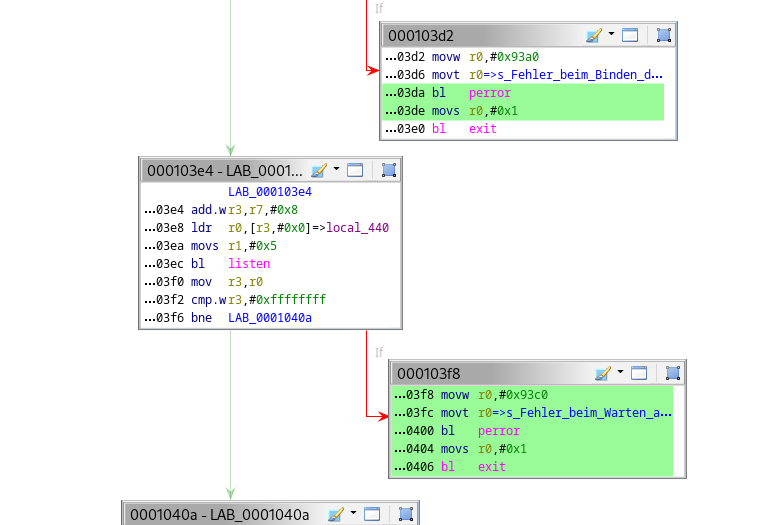
\includegraphics[width=\linewidth]{img/basic-blocks-example}}
    \caption{Zeigt ein Beispiel mehrerer basic blocks. Der hier gezeigte Disassembly und der damit verbundene
    Kontrollflussgraph entstammt dem selbst implementierten \gls{tcp}-Servers aus dem Kapitel \ref{subsubsec:persistent-mode}.
    Verwendet wurde hierbei das Reverse-Engineering-Tool Ghidra.}\label{fig:basic-block}
\end{figure}\\
Ein basic block ist dadurch gekennzeichnet, dass die erste Instruktion als Einstiegspunkt (\textit{entry point}) und die letzte Instruktion
als Ausstiegspunkt (\textit{exit point}) bezeichnet wird.
Ein entry point ist in der Regel die erste Instruktion nach einem Sprung im Codesegment.
Der exit point kann das Ende des Codes oder eine Sprunginstruktion im Codesegment sein.
Die Verbindung zweier basic blocks (in Abbildung~\ref{fig:basic-block} mit Pfeilen dargestellt) wird als \textit{branch edge} bezeichnet.
in dieser Arbeit wird ein Pfad von mehreren miteinander verbundenen basic blocks als Codepfad bezeichnet. \\
\linebreak
Der Programmcode wird klassischerweise zuerst mit dem von \gls{afl} bereitgestellten custom compiler \texttt{afl-cc} kompiliert.
In diesem Schritt wird das Programm von \gls{afl} auf bedingte Sprünge untersucht und an jeder Instruktion wird eigener
Programmcode an diesen Stellen injiziert.
Anschließend wird der dabei entstandene Programmcode kompiliert und ist somit für die Fuzzing-Kampagne vorbereitet. \\
\linebreak\linebreak
Zur Optimierung der Fuzzing-Kampagne kann der Korpus nach dem ersten Durchlauf mit einem weiteren Tool von \gls{afl}
(\texttt{afl-cmin}) minimiert werden.
Bei der Minimierung des Korpus wird darauf geachtet, ob beim Ausführen des Programms neue Programmpfade traversiert werden.
Danach wird die Fuzzing-Kampagne mit dem Tool \texttt{afl-fuzz} gestartet.
Dabei werden in einem Testdurchlauf zuerst alle gesammelten Inputs auf ihre Validität geprüft, indem \gls{afl} darauf
achtet, ob das zu untersuchende Programm in einen definierten Zustand gelangt und fehlerfrei terminiert.
Zusätzlich wird geprüft, welche Programmpfade abgelaufen werden und ob Testfälle neue Programmpfade erreichen.
Diese Strategie bezeichnet man als covered-based Strategie~\cite[vgl.][7]{iot-fuzzing}.\\
\linebreak
Nachdem alle Testfälle erfolgreich durchgeführt wurden, beginnt die Mutation des Inputs.
Hierzu gibt es auch verschiedene Ansätze, die von Fuzzern verfolgt werden.\\
Ein elementarer Bestandteil des \gls{afl} ist der darin enthaltene Forkserver.
Dieser ist für die Vorbereitung des Binaries für die Fuzzing-Kampagne verantwortlich.
Das Binary durchläuft den Syscall \texttt{execve()} einmalig, welcher dafür verantwortlich ist, das zu startende Programm in
den aktuellen Prozess zu laden.
Zudem ist der Forkserver dafür verantwortlich sicherzustellen, dass das zu instrumentierende Programm nur ein Mal
zum Ausführen gelinkt wird und ein Einsprungspunkt für den Fuzzer nach der Initialisierung gesetzt wird.
An diesem Einsprungspunkt werden nach der Initialisierung die Instruktionen -- oder auch Testcases -- der Fuzzing Kampagne von \gls{afl}
injiziert.
Dadurch wird die Performance verbessert, da das Programm bei mehrfacher Ausführung nur jeweils ein Mal initialisiert wird
und der ursprüngliche Zustand des Prozesses wiederhergestellt wird.
Anschließend werden Kopien des Prozesses an der Stelle des Forkservers mithilfe des \texttt{fork()} Syscalls erstellt.
Daher stammt auch der Name Forkserver.
Er setzt einen Startpunkt für den Fuzzer fest, an dem der Prozess des Programms in dem zu der Zeit feststehenden Zustand
mithilfe des \texttt{fork()} Syscalls kopiert wird.
Dieser Prozess wird auch \textit{Forken} genannt.
Dabei entsteht eine logische Einteilung der beiden Prozesse wobei der Elternprozess der Prozess ist, welcher vor dem Forken
bereits vorhanden war.
Der aus dem Forken entstandene Prozess heißt Kindprozess.\\
\linebreak
Die von \gls{afl} genutzte Syntax besteht aus drei Komponenten.
%! Author = chaorn
%! Date = 17.02.24

\begin{lstlisting}[language=bash, caption={Syntax des AFL Fuzzing-Befehls},label={lst:afl-synthax}]
$ afl-fuzz -i in/ -o out/ -- /app/mmapp @@
\end{lstlisting}
Man beginnt mit dem Tool \texttt{afl-fuzz}.
Daraufhin wird das Flag \texttt{-i} mit dem Pfad zum Ordner (hier~\ref{lst:afl-synthax}: \textit{in/}) gesetzt, der den Korpus enthält.
Anschließend daran wird das Flag \texttt{-o} mit dem Pfad zu dem Ordner (hier~\ref{lst:afl-synthax}: \textit{out/}) gesetzt,
in dem die zur Laufzeit der Fuzzing-Kampagne generierten Ergebnisse abgelegt werden.
Zur besseren Lesbarkeit kann nach dem letzten Ordner ein \textit{- -} angefügt werden.
Danach wird der Pfad zur zu untersuchenden Applikation angegeben.
Zuletzt wird die Art der Übermittlung des Inputs dem Binary beschrieben.
Die Zeichen \texttt{@@} stehen für die Kommunikation mit dem Binary mit Dateien.
Die Zeichen dienen als Platzhalter für \gls{aflpp} und werden zur Laufzeit des Fuzzers mit den generierten Daten mit dem
Namen \textit{.curr\_input} ersetzt ~\cite{afl-file-extension}.
Dadurch werden ganze Dateien an das zu untersuchende Binary übergeben.
Wenn man jedoch das \texttt{@@} weglässt, so wird der Inhalt der im Input-Verzeichnis enthaltenen Dateien sequentiell an
das Binary über stdin übergeben. \\
\linebreak
In dieser Arbeit wird ausschließlich \gls{aflpp} verwendet.
\gls{aflpp} ist eine Abzweigung von \gls{afl} und wird von einer breiten Community erweitert und verbessert.
\gls{afl} und \gls{aflpp} unterscheiden sich maßgeblich in der Effizienz der Mutation, der Entdeckung von Codepfaden und
einigen in \gls{afl} nicht umgesetzten Features.
Zur VereinfachungIn wird in den folgenden Kapiteln nur von \gls{afl} als Abkürzung für \gls{aflpp} gesprochen.